\documentclass[10pt]{article}

\usepackage{multicol}
\usepackage{geometry}
\geometry{bottom=4em,top=6em, inner=2.2cm, outer=4em,  headheight=\paperheight}
\usepackage[export]{adjustbox}
\usepackage{array}
\usepackage{amsmath}
\usepackage{amsfonts}
\usepackage{fancyhdr}
\usepackage{lastpage}
\usepackage{xcolor}
\usepackage{enumitem}
\usepackage{pifont}
\usepackage{graphicx}
\graphicspath{{../img}}
\usepackage{pgfplots}
\pgfplotsset{compat=1.18}
\usepackage{tabularx}
\usepackage{polynom}
\usepackage{setspace}
\usepackage{pdfpages}
\usepackage{tikz}
\usetikzlibrary{angles,quotes}
\setlist{nosep}

\pagestyle{empty}

\begin{document}

\begin{center}
{\Large\textbf{Algebra II Regents Cheat Sheet: Normal Distribution}}
\end{center}

\hrule
\vspace{0.5em}

\textbf{Normal Distribution}

\begin{itemize}
    \item Bell-shaped and symmetric.
    \item Mean = Median = Mode.
    \item Centered at the mean $\mu$.
    \item Spread is measured by the standard deviation $\sigma$.
\end{itemize}

\vspace{0.5em}

\textbf{Notation}

\[
\mu = \text{mean}
\]

\[
\sigma = \text{standard deviation}
\]

\[
\mu \pm \sigma
\quad
\mu \pm 2\sigma
\quad
\mu \pm 3\sigma
\]

represent points 1, 2, and 3 standard deviations from the mean.

\vspace{0.5em}

\textbf{Empirical Rule (68--95--99.7 Rule)}

\[
\begin{array}{c|c}
\text{Interval} & \text{Percent of Data} \\ \hline
\mu \pm \sigma & 68\% \\
\mu \pm 2\sigma & 95\% \\
\mu \pm 3\sigma & 99.7\%
\end{array}
\]

\vspace{1em}

\textbf{Useful Breakdown}

\[
\begin{array}{c|c}
\text{Region} & \text{Percent} \\ \hline
\mu \text{ to } \mu+\sigma & 34\% \\
\mu+\sigma \text{ to } \mu+2\sigma & 13.5\% \\
\mu+2\sigma \text{ to } \mu+3\sigma & 2.35\% \\
\text{Beyond } \mu+3\sigma & 0.15\%
\end{array}
\]

(The same percentages occur on the left side by symmetry.)

\vspace{1em}

\textbf{Normal Curve Diagram}

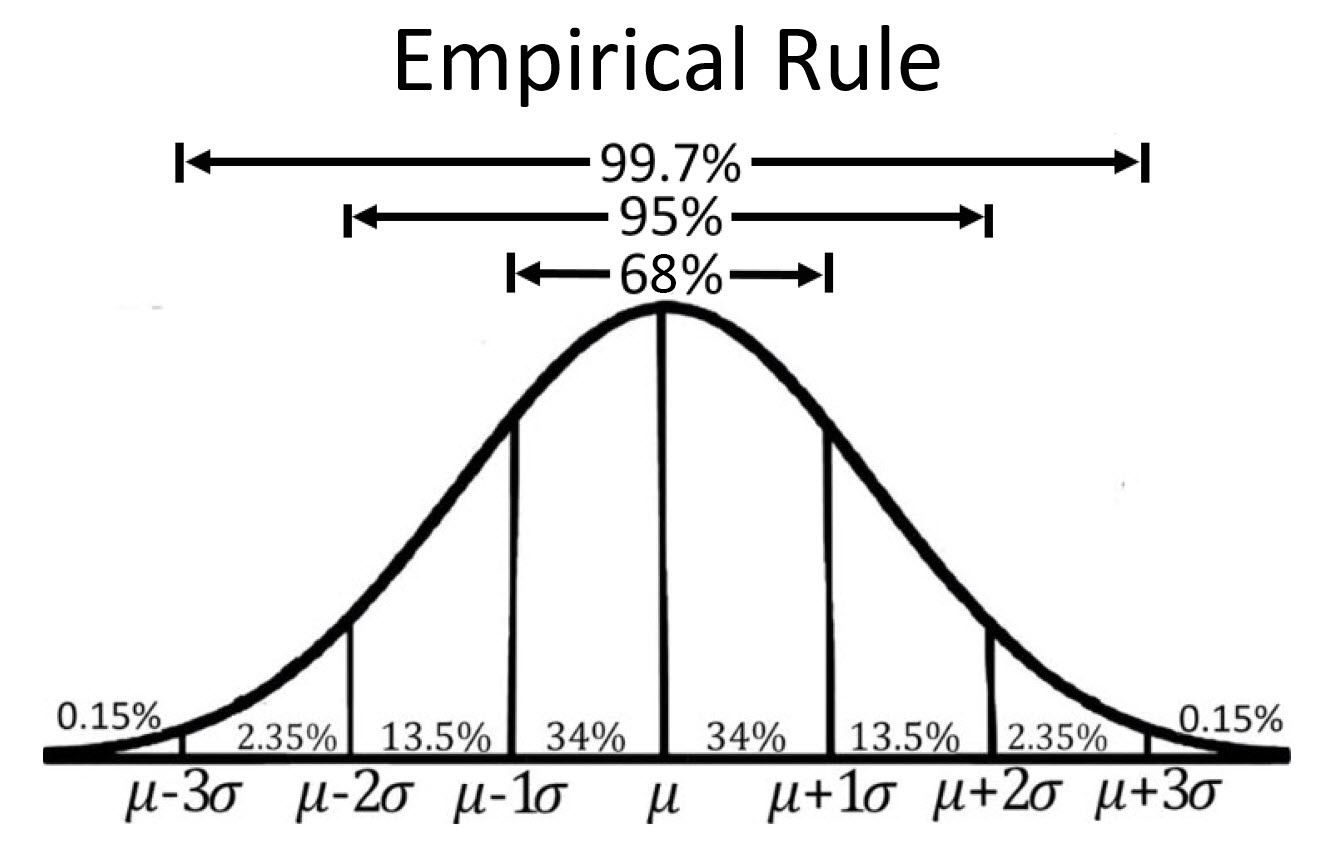
\includegraphics[width=0.8\textwidth]{empirical-rule-normdist2.jpg}

\end{document}